% !TEX root = main.tex
\section{Modello}
\label{sec:modello}

\subsection{Introduzione}
\label{set:introduzione}
Il modello implementato rappresenta una variante dell'architettura proposta da Carlos Bentancour e Wen-Hui Chen nell'articolo "Deep reinforcement learning for portfolio management of markets with a dynamic number of assets"~\citep{betancourt2021deep} adattata al mercato azionario "S\&P500". L'innovazione principale di questa architettura risiede nella proprietà DNA (Dynamic Number of Assets), ovvero una struttura che permette di operare su mercati finanziari in cui il numero di asset varia nel tempo. Questa caratteristica ha determinato la scelta dell'architettura per l'implementazione on-device: essa consente infatti all'utente di selezionare un paniere arbitrario di titoli e calcolarne l'allocazione ottimale dei pesi in fase di inferenza, senza richiedere una fase di riaddestramento specifico sui singoli asset scelti. 

\subsection{Feature}
\label{set:feature}
Le feature date impasto al modello sono di 3 tipi diversi
\subsubsection{Feature per asset}
Sono le uniche feature che passano dalla GRU. Vengono passate per ogni asset e per ogni giorno della sliding window, sono \textbf{high, low, close, VIX}.
Le prime tre servono per leggere la volatilità e il trend recente di ogni titolo.
VIX è un dato di mercato, è identico per tutti i titoli nella stessa data, passa sia dalla GRU ma anche come scalare globale in \textbf{risk\_state} arrivando alle teste sia filtrato sia grezzo.
Forma: $(B, N, 30, 4)$ dove $B$ è la dimensione del batch, $N$ è il numero di asset nel paniere, $30$ la dimensione della finestra scorrevole e $4$ le features in input.
\subsubsection{Normalizzazione}
Ogni osservazione è una finestra scorrevole di $W=30$ giorni di contrattazione.
Le tre serie storiche di prezzo (high, low, close) vengono normalizzate dividendo
ciascun valore per l’ultimo prezzo di chiusura della finestra di osservazione in modo da renderli dei rapporti puri.
La normalizzazione è necessaria per tre motivi.
In primo luogo serve perché i livelli di prezzo assoluti crescono di ordini di grandezza tra il periodo di addestramento e quello di test, se non normalizzassimo gli input essi risulterebbero fuori scala.
In secondo essa serve a mantenere l'equità dell'aggregazione, dato che il contesto di mercato è la media permutation-invariant degli embedding per-asset se tenessimo i prezzi grezzi essi andrebbero a distorcere il segnale di esposizione.
Infine serve perché la valutazione su panieri diversi da quello di addestramento richiede input privi di unità di misura.

Il VIX è riscalato a scala fissa (/100), questa normalizzazione
a scala fissa evita di introdurre informazione dipendente dal futuro,
poiché non viene stimata alcuna media o deviazione sull’intero campione.

\subsubsection{prev\_weights (B, N)}
La composizione attuale del portafoglio prima di agire: una percentuale per ogni asset che somma a 1. Alla rete però viene data come feature solo la quota CASH attuale in quanto la selezione dei titoli normali è sempre equal-weight.
\subsubsection{risk\_state (B, 6)}
Sei scalari globali (identici per ogni asset) che indicano lo stato di rischio dell'agente (i primi 3) e del mercato nel suo insieme.
\begin{enumerate}
    \item \textbf{Drawdown corrente}: Misura la perdita percentuale rispetto al massimo storico del capitale nel'episodio. Serve all'agente per capire quanto sta perdendo rispetto al picco inducendo a ridurre l'esposizione se la strategia sta soffrendo. 
        \begin{itemize}
    \item \textit{Trasformazione}: $\frac{\textit{picco} - \text{valore}}{\text{picco}}$
    \item \textit{Range}: $[0.0, 1.0]$
  \end{itemize}
    \item \textbf{Volatilità del portafoglio}: deviazione standard annualizzata dei rendimenti del portafoglio a 21 giorni (un mese), misura il rischio specifico delle scelte di allocazione correnti dell'agente.
       \begin{itemize}
    \item \textit{Trasformazione}: $\ln(1+ \sigma_{ann})$
    \item \textit{Range}: $[0.0, 1.0]$
  \end{itemize}
    \item \textbf{Tempo sott'acqua}: numero di giorni consecutivi senza raggiungere un nuovo picco del capitale, aiuta l'agente a capire se il portafoglio è bloccato in una fase di stallo prolungata o se recupera velocemente
    \begin{itemize}
    \item \textit{Trasformazione}: $\ln(1+ \frac{giorni}{252})$
    \item \textit{Range}: $[0.0,1.5]$
  \end{itemize}
    \item \textbf{Volatilità di mercato compressa}: volatilità storica a 21 giorni del paniere (tutti i titoli), da il contesto macroeconomico permettendo di distringuere tra mercati calmi e mercati volatili
    \begin{itemize}
    \item \textit{Trasformazione}: $\ln(1+\sigma_{mkt\_ann})$
    \item \textit{Range}: $[0.0, 0.8]$
  \end{itemize}
    \item \textbf{Livello del vix}: l'indice VIX della volatilità attesa a 30 giorni, fornisce una misura di aspettativa futura
    \begin{itemize}
    \item \textit{Trasformazione}: $\frac{VIX}{100}$
    \item \textit{Range}: $[0.1, 0.8]$
  \end{itemize}
    \item \textbf{Volatilità di mercato grezza}: uguale all'altra ma non in scala logaritmica, permette al modello di percepirte direttamente l'intensità degli shock del mercato senza smorzarli.
    \begin{itemize}
    \item \textit{Trasformazione}: $\min(\max(\sigma_{mkt\_ann},0), 3.0)$
    \item \textit{Range}: $[0.0,3.0]$
  \end{itemize}
\end{enumerate}



\subsection{Architettura}
\label{set:architettura}
L'intera architettura è stata progettata per funzionare con un numero qualsiasi di asset, in qualsiasi ordine. 
Questo risultato è ottenuto con due proprietà:
\begin{itemize}
  \item \textbf{Permutation-equivariance}: la stessa rete è applicata ad ogni asset indipendentemente (i pesi sono condivisi), cioè scambiare due asset scambia solo i loro output
  \item \textbf{Permutation-invariance}: il contesto di mercato si ottiene con una media sugli asset, non dipende da quanti sono nè da come sono ordinati
\end{itemize}

Per convenzione il CASH cioè la liquidità è sempre l'ultimo asset lungo l'asse 1.

\subsubsection{Rete}
La rete del modello presenta un'architettura Actor-Critic. 
Ogni giorno comprime lo storico di ogni asset con una GRU condivisa facendone la media in modo da ottenere un contesto di mercato indipendente dal numero di asset.
Da lì produce la sua decisione indicando quanto esporsi al mercato, ovvero gestisce quanto parte del portafoglio viene investita (equal-weight per gli asset) e quanta parte rimane in contanti. 
La rete si divide in sei componenti fondamentali, riassunti nel diagramma di Fig.~\ref{fig:architettura}.

\begin{figure}[h]
\centering
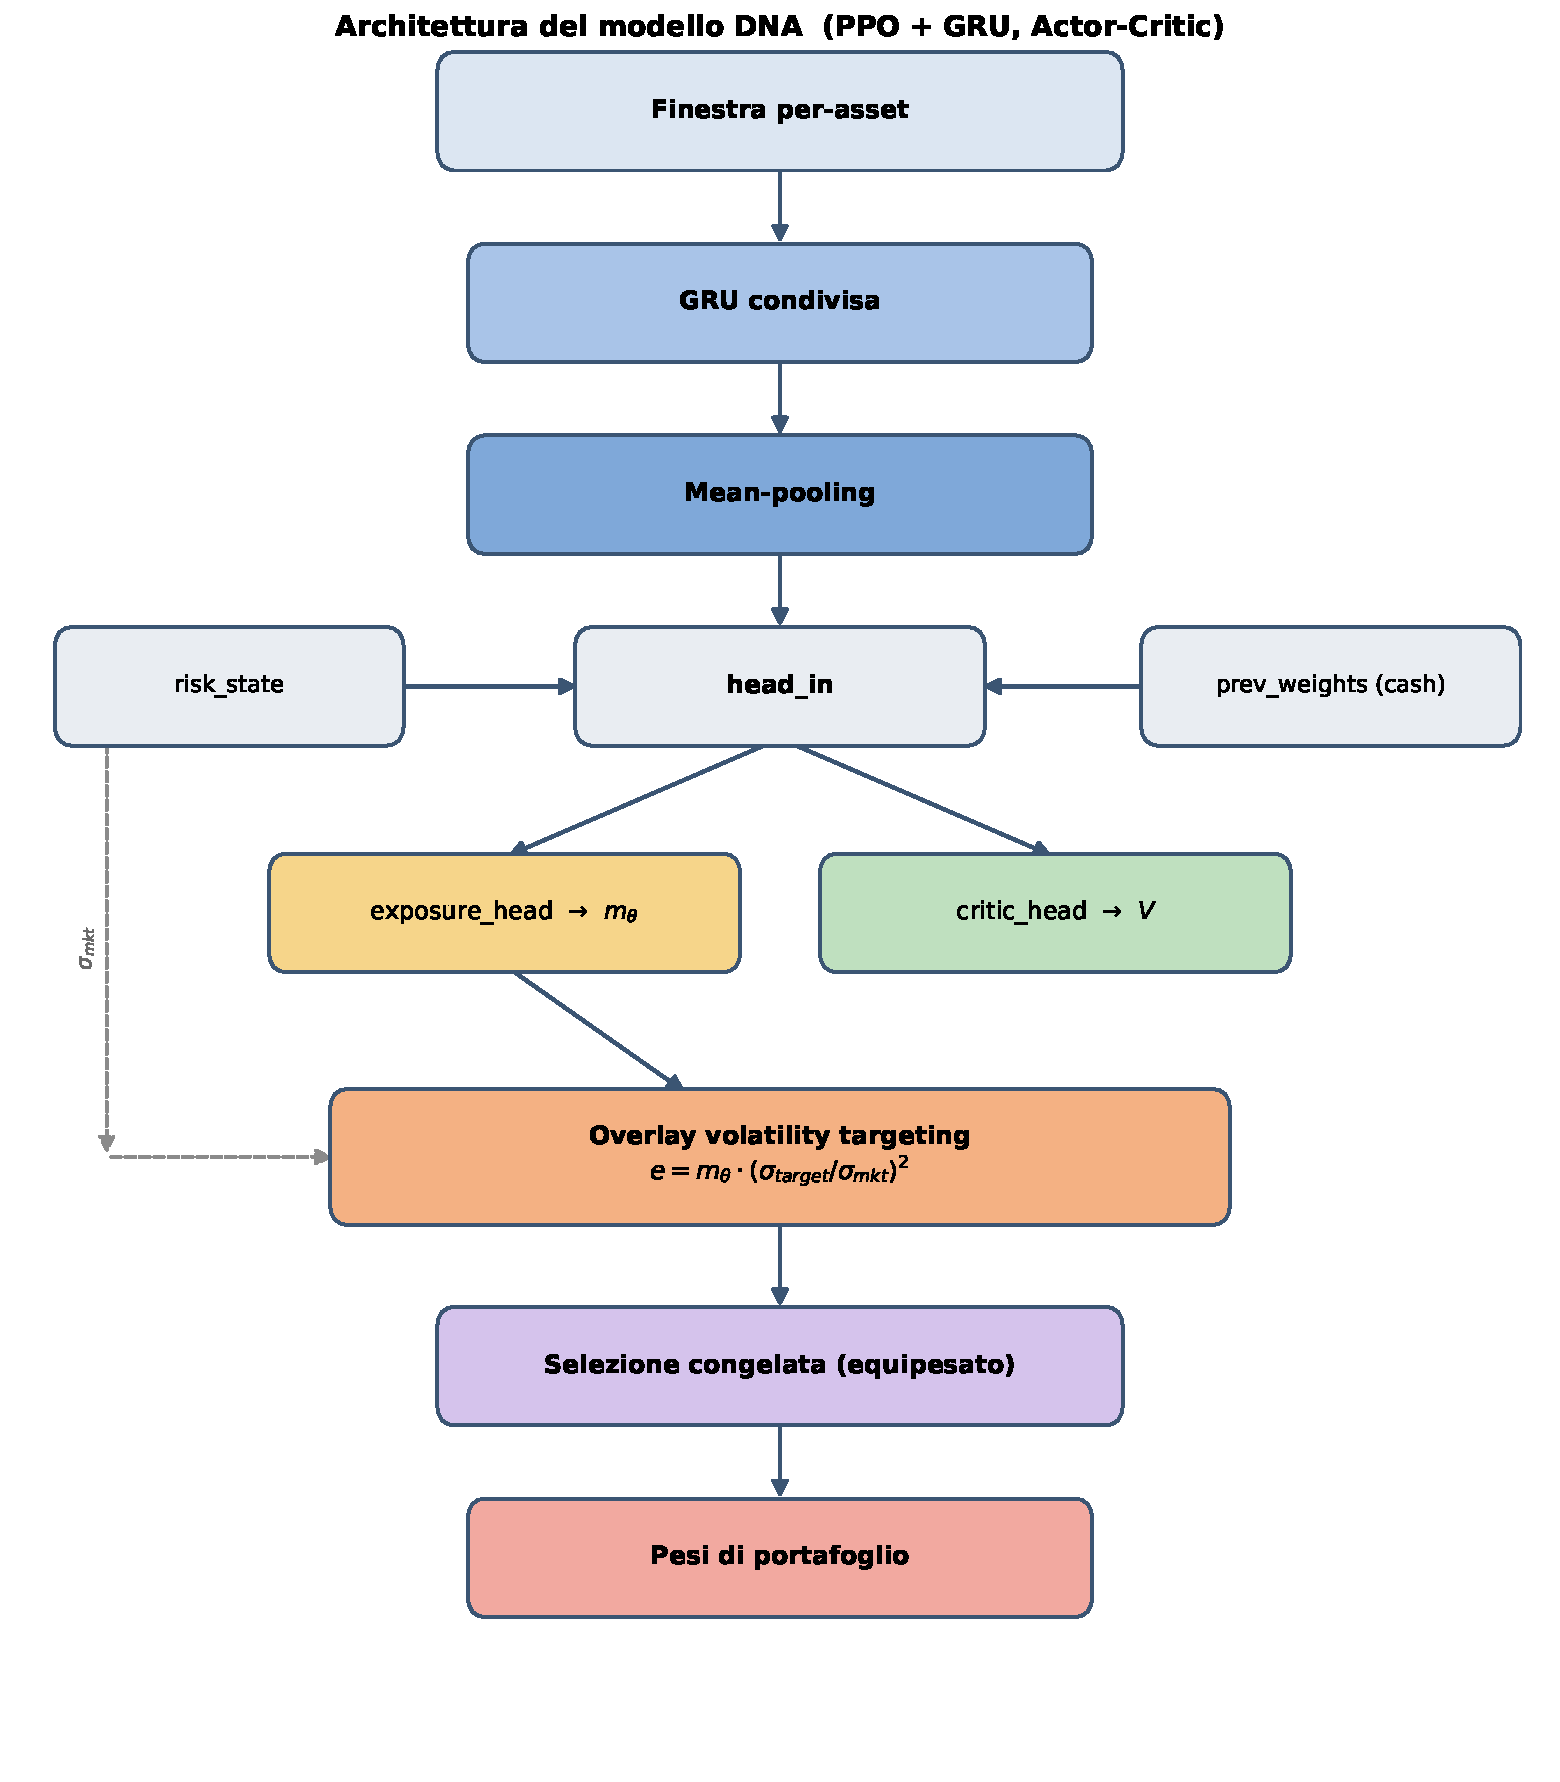
\includegraphics[width=0.8\textwidth]{architettura.pdf}
\caption{Architettura del modello: dalla finestra per-asset, tramite GRU condivisa e mean-pooling, al vettore \lstinline{head_in} (con \lstinline{risk_state} e \lstinline{prev_weights}), fino all'overlay di volatility targeting e ai pesi di portafoglio.}
\label{fig:architettura}
\end{figure}

Prima di effettuare qualunque operazione avviene la fase di normalizzazione descritta poco sopra, in seguito questi dati vengono passati alla GRU.
\paragraph{GRU}
Riceve features della forma $(B, N, 30, 4)$ e applica un reshape che fonde \textbf{B} e \textbf{N} in un'unica dimensione di taglia $B\times N$, usata come nuovo batch della GRU. In questo modo ogni asset di ogni campione diventa un esempio indipendente processato dalla stessa identica GRU: in sostanza c'è una sola GRU applicata a ciascuno degli $N$ asset.
La struttura interna della GRU è composta da 2 layer impilati, \lstinline{hidden_size=10}, \lstinline{batch_first=True}.
\begin{itemize}
  \item Layer 1: input 4 feature → 10 hidden.
  \item Layer 2: 10 → 10.
\end{itemize}
 
Si prende in seguito solo l'ultimo timestep ovvero un vettore di 10 elementi contenente una sintesi appresa della dinamica recente dell'asset. 
Ora abbiamo un embedding per ogni asset, poiché la stessa rete è applicata a ciascun asset in modo indipendente, l'embedding di ciascuno dipende solo dalla sua serie storica, non da chi gli sta accanto nè dalla sua posizione nella lista. 
Quindi scambiando due asset in input gli embedding si spostano insieme ai loro asset. 
È ancora presente l'equivarianza.
Dopo aver ottenuto gli embedding ne calcoliamo la media per ottenere il contesto di mercato.
\begin{lstlisting}[language=Typescript]
context = last_hidden.mean(dim=1)
\end{lstlisting}
La media è un'operazione simmetrica quindi il \lstinline{context} sarà identico qualunque sia l'ordine degli asset in questo modo otteniamo l'invarianza. 
L'invarianza ci permette di utilizzare il modello su qualsiasi asset non solo quelli su cui è stato addestrato. 
Anche se la media ci fa perdere la capacità di distinguere i singoli asset possiamo usarla in quanto, decidere quanto esporsi al mercato è una proprietà del portafoglio nel suo insieme e non deve dipendere da un'ordinamento arbitrario

\paragraph{Actor}
Nel modello l'Actor non si occupa di scegliere direttamente l'esposizione, ma produce un unico moltiplicatorre appreso $m_\theta$ che andrà poi a correggere una formula fissa di volatility targeting. 
Riceve in input un vettore da 17 elementi, ottenuto concatenando il contesto di mercato (i 10 numeri in output della GRU), il \lstinline{risk_state} del portafoglio e la quota di cash attuale:

\begin{lstlisting}[language=Typescript, caption={Struttura della testa di esposizione}]
exposure_head = Sequential(
    Linear(17 -> 16), ReLU, Linear(16 -> 1)
)
m_theta = softplus(exposure_head(input))   # m_theta > 0
\end{lstlisting}

L'output della exposure head passa poi in una \lstinline{softplus} che garantisce $m_\theta > 0$.
Il bias dell'ultimo layer è inizializzato in modo che al passo zero $\text{softplus}(\text{bias})=1$. 
Quindi il modello parte con $m_\theta \approx 1$, cioè come volatility targeting puro. I pesi del layer sono inoltre scalati di un fattore $0.1$ in questo modo la parte da appredere cresce lentamente invece di dominare da subito con valori casuali. In sostanza l'unico grado di libertà appreso della decisione è una correzzione moltiplicativa attorno a $1$ sopra una regola deterministica.

\paragraph{Overlay di volatility targeting}
È il componente che trasforma il moltiplicatore appreso $m_\theta$ nella decisione di esposizione $e_t$, applicando la formula di volatility targeting descritta nella metodologia (Sez.~\ref{sec:metodi}). 
Una volta ottenuta $e_t$ la selezione degli aset è congelata a equal weight e la liquidità riceve $1- e_t$.
L'ordine con cui elenchiamo i titoli non conta. Infatti se invertiamo la posizione di due asset all'ingresso del modello, anche i rispettivi pesi in uscita si scambieranno di posto, senza alterare la decisione finale.

\paragraph{Critic}
Il Critic serve unicamente durante l'addestramento come baseline per il calcolo del vantaggio in PPO.
Fornisce all'algoritmo PPO una stima del valore dello stato che serve a rendere l'apprendimento più stabile. 
Ha la stessa struttura della \lstinline{exposure_head} e riceve lo stesso identico input da 17 elementi:
\begin{lstlisting}[language=Typescript, caption={Struttura del critic}]
critic_head = Sequential(
    Linear(17 -> 16), ReLU, Linear(16 -> 1)
)
\end{lstlisting}

L'output è un singolo scalare $V(s)$ che rappresenta la stima del ritorno atteso a partire dallo stato corrente. 
Questo valore viene usato da PPO come baseline nel calcolo del vantaggio: invece di aggiornare la policy in base al ritorno grezzo $R_t$ si usa infatti il vantaggio $A_t = R_t - V(s_t)$ che misura quanto meglio del previsto è andata l'azione. 
Sottrare $V(s_t)$ riduce la varianza del gradiente e quindi rende l'addestramento più stabile e veloce. 

\paragraph{Output del modello}
Il modello restituisce in output il vettore dei pesi di portafoglio \[
w = \big[\, \underbrace{e_t/(N-1),\ \dots,\ e_t/(N-1)}_{N-1\ \text{asset rischiosi}},\ \underbrace{1 - e_t}_{\text{cash}} \,\big],
\] dove $e_t$ è l'esposizione prodotta dall'overlay vol targeting. È una distribuzione che somma a 1, con ultimo elemento la liquidità e gli asset tutti allo stessto peso.

\subsection{Environment}
L'ambiente \lstinline{PortfolioEnv} implementa la simulazione di mercato con cui l'agente interagisce. 
A ogni step (un giorno di borsa) gli fornisce un'osservazione, riceve un'azione, esegue il ribilanciamento tenendo conto dei costi, fa evolvere il valore del portafoglio e calcola la ricompensa.


Lo stato che l'agente riceve a ogni step è composto da tre elementi:
\begin{itemize}
    \item \textbf{feature di mercato} per ogni asset (la finestra di 30
    giorni di \lstinline{high, low, close, vix}), che passano per la GRU;
    \item \textbf{pesi correnti} del portafoglio \lstinline{prev_weights};
    \item \textbf{stato di rischio} \lstinline{risk_state}, sei scalari
    globali (uguali per tutti gli asset) che descrivono la salute del portafoglio e il regime di
    mercato.
\end{itemize}
La volatilità e il tempo in drawdown sono compresse con $\log(1+x)$ per fare in modo che pochi eventi estremi non possano pesare troppo nell'osservazione, il drawdown resta lineare.


Una volta ricevuti i nuovi \lstinline{prev_weights} , l'ambiente li applica attraverso due passaggi. 
Prima calcola i costi di transazione legati al ribilanciamento, poi aggiorna il valore del portafoglio applicando i prezzi di mercato del giorno corrente.
Da questo ricalcolo si ricavano il rendimento giornaliero, il nuovo massimo storico raggiunto e il drawdown attuale. 
Infine, la volatilità di mercato impiegata nel \lstinline{risk_state} e nell'overlay non è una variabile esterna fornita dal dataset, ma un segnale calcolato internamente. 
Essa è la deviazione standard mobile dei rendimenti a 21 giorni del paniere equipesato, riscalata su base annua ($\times\sqrt{252}$).

\paragraph{Costi di transazione (\lstinline{TransactionOptimizer})}
Nella realtà ogni operazione di mercato prevede il pagamento di commissioni.
Passare dalla composizione attuale del portafoglio $w'$ ai nuovi pesi desiderati $w$ richieda di comprare e vendere titoli.
Anche nell'ambiente simulato è stato fatto in modo che per ogni transazione si paghi una commissione dello $0{,}2\%$.
Questo costo viene quantificato tramite un fattore di rimanenza $\mu \in (0,1]$, che rappresenta la quota di capitale effettivamente intatta dopo aver pagato i costi: $V_{\text{post}} = \mu\, V_{\text{pre}}$. 
Il valore di $\mu$ è definito dall'equazione:\begin{equation}\mu = 1 - \sum_i \Big[\, b_i \max(\mu\,p_i - p'_i,\,0) + s_i \max(p'_i - \mu\,p_i,\,0)\,\Big],\end{equation}
dove $p_i$ e $p'_i$ sono le quote target e correnti del titolo $i$, mentre $b_i$ e $s_i$ indicano le commissioni per acquisti e vendite.
Il capitale finale $\mu$ dipende dal ricavo ottenuto vendendo i vari titoli a cui vengono sottratti i costi di commissione, l'ammontare delle commissioni però dipende a sua volta dal capitale finale.
Questo problema è stato risolto tramite una serie di iterazioni a punto fisso adottando lo schema proposto da Jiang et al.~\cite{jiang2017deep}. Anche nel modello originale della DNA~\cite{betancourt2021deep} sono applicati i costi di transazione, ma vengono calcolati attraverso un programma lineare (LP). 
Si è scelto di implementare i costi di transazione con un metodo di iterazione a punto fisso perché in questo modo è stato possibile trasferire il modello on-device nell'applicazione.
Includere questi costi impedisce alla rete di ottenere facili guadagni teorici attraverso un continuo ribilanciamento e garantisce che il risultato sia il più simile possibile a una situazione reale.

\paragraph{Episodio e ricompensa}
Un episodio non ha lunghezza fissa, esso parte
da un giorno estratto a caso e prosegue fino all'ultimo giorno del periodo di
addestramento. La durata varia quindi da un minimo
garantito di 252 giorni di borsa (circa un anno) fino all'intero orizzonte di training. 
A ogni passo l'ambiente restituisce la ricompensa, la cui
forma è discussa nella sezione sulla metodologia (Sez.~\ref{sec:metodi}).


\paragraph{Provenienza}
Il termine base di log-rendimento è la scelta standard nel portfolio management
con reinforcement learning . I due termini di penalità non derivano invece
da un singolo lavoro di letteratura, ma sono un reward shaping progettato
appositamente per questo modello: sono la traduzione, nella funzione obiettivo,
dell'idea che la difesa debba attivarsi quando il rischio di mercato aumenta.
L'overlay su cui la reward agisce è a sua volta l'analogo appreso del volatility
targeting~\cite{moreira2017volatility}.

\subsection{Addestramento}
Il modello è stato addestrato con \textbf{Proximal Policy Optimizaton} (PPO), un algoritmo di reinforcement learning on-policy della famiglia Actor-Critic~\cite{schulman2017proximal}. L'addestramento alterna una fase di raccolta di esperienza ottenuta facendo interagire la policy corrente con l'ambiente, con il successivo aggiornamento dei pesi in base ai dati raccolti.

\paragraph{Algoritmo di addestramento (PPO)}
L'addestramento segue uno schema iterativo suddiviso in tre fasi:
\begin{enumerate}
    \item \textbf{Raccolta dell'esperienza:} a ogni ciclo, l'agente interagisce simultaneamente con \lstinline{n_envs} ambienti di mercato indipendenti, registrando una traiettoria di \lstinline{n_steps} passi temporali per ciascuno.

    \item \textbf{Valutazione delle decisioni (Advantage):} il vantaggio $A_t$ di ogni azione è stimato con la Generalized Advantage Estimation (GAE)~\cite{schulman2016gae}, ovvero lo scarto tra il rendimento ottenuto e quello previsto dal Critic (cfr. Cap.~\ref{chap:backgrounds}).

    \item \textbf{Aggiornamento prudente della policy:} i pesi sono aggiornati massimizzando l'obiettivo clippato di PPO, che limita l'ampiezza di ogni singolo aggiornamento e la divergenza della strategia (cfr. Cap.~\ref{chap:backgrounds}).
\end{enumerate}

La funzione di perdita complessiva combina la loss della policy con l'errore di stima del Critic (pesato dal coefficiente \lstinline{vf_coef}). 
L'ottimizzazione viene  eseguita con l'algoritmo Adam su minibatch, applicando un vincolo sul gradiente per impedire oscillazioni numeriche distruttive lungo le \lstinline{n_epochs} passate sui dati.
La catena che lega il tutto è: 
 
la reward si accumula nel ritorno $R_t$; il Critic prova a prevederlo con $V(s)$; la differenza è il vantaggio; il vantaggio entra nella loss che spinge l'Actor a ripetere le azioni con vantaggio positivo.

\paragraph{Esplorazione}
Dato che la selezione è congelata e l'unica decisione appresa è l'esposizione, PPO
esplora campionando solo l'esposizione da una distribuzione Beta.
La rete produce un valore di esposizione deterministico, la policy è la Beta centrata su quel valore, che permette all'agente di esplorare valori di esposizione vicini.
L'ampiezza dell'esplorazione è regolata da un parametro appreso $\kappa$, così la rete decide da sola quanto esplorare.
In inferenza il campionamento è rimosso: la policy diventa deterministica e coincide con l'esposizione prodotta dalla rete.

\paragraph{Dati e suddivisione temporale}
L'addestramento avviene su un paniere di 8 large-cap
(\lstinline{CAT DIS HD IBM JNJ JPM PG UNH}) con finestra di osservazione di 30
giorni. 
Sono stati scelti solo 8 titoli perché esperimenti preliminari hanno dimostrato che usare un paniere più ampio durante l'addestramento non migliora le performance ma rende il modello meno cauto nella geestione dell'esposizione. 
 I dati sono divisi cronologicamente per evitare qualsiasi lookahead:
addestramento sul periodo 2000--2012, validazione 2012--2015, e test fuori campione dal 2015 in poi. Grazie all'invarianza per permutazione e
all'N-agnosticismo, il modello allenato su questo paniere può poi essere valutato
zero-shot su universi diversi.

\paragraph{Iperparametri}
\begin{center}
\begin{tabular}{lc}
\toprule
Iperparametro & Valore \\
\midrule
Ambienti paralleli (\lstinline{n_envs})        & 8 \\
Passi per rollout (\lstinline{n_steps})        & 128 \\
Epoche per aggiornamento (\lstinline{n_epochs})& 5 \\
Dimensione minibatch                           & 256 \\
Passi totali di training                       & 700\,000 \\
Fattore di sconto $\gamma$                     & 0.9 \\
$\lambda$ della GAE                            & 0.95 \\
Raggio di clipping $\epsilon$                  & 0.2 \\
Peso value loss (\lstinline{vf_coef})          & 0.5 \\
Coeff. entropia (\lstinline{ent_coef})         & 0 \\
Learning rate (Adam)                           & $3\times10^{-4}$ \\
Norma massima del gradiente                    & 0.5 \\
Concentrazione iniziale $\kappa$               & 50 \\
\bottomrule
\end{tabular}
\end{center}

